\documentclass{paper}

\usepackage{lipsum}

\usepackage{graphicx}
\usepackage{float}

\begin{document}

\begin{titlepage}
	\begin{center}
		\huge{\bfseries Apache Spark} \\
		\line(1,0){200} \\
		[1.5cm]
		\textsc{\LARGE Technology Paper for I524}\\
		[14cm]
	\end{center}
	\begin{flushright}
	\textsc{\large Saurabh Swaroop \\
	HID-SP18-522 \\
	March 20, 2018 \\}
	\end{flushright}

\end{titlepage}

\tableofcontents

\thispagestyle{empty}
\cleardoublepage

\setcounter{page}{1}

\section{Introduction}\label{sec:intro}
The amount of data consumed and generated by enterprise are huge in current world. Such large volume of data has created a necessity for the companies to make the best use of the diversity and hidden information associated with them.Not only these informations improvise the productivity but enables enterprises to identify new opportunities.With the advent of big data, more enterprises are incorporating data analytics when building strategic applications and making decisions. Data processing and its effective analysis plays a very important role in functioning and getting ahead of the competition for almost every enterprise now a days. \hfill\break


Enterprise need to have a standard process and infrastructure to perform data analysis which involves
several stages like Data Collection, Data Cleaning, Data Storage, Data Processing, Data Analysis. On top of these stages lies the models on which enterprise map their business to get ahead of their peers.\hfill\break

Apache Spark is cluster computing framework which is used for data processing and analysis over large scale with great processing rate.

\newpage
\section{Spark Overview}

Spark is an Apache open source project originally developed in AMPLab at UC Berkeley. It is a cluster computing framework which is built on top of Hadoop distributed file system HDFS for data analysis and processing. Unlike Hadoop, Spark does not use Map-reduce engine to read and write to hard disk. It is based on, in memory computation process which increases its speed over 100X as compared to Hadoop.\hfill\break


In memory cluster computing framework allows applications to load data into a cluster?s memory. This process enables multiple recursive queries without performance overhead. It allows both batch and real-time data analytic and processing pay loads.\hfill\break


Spark is available for Linux, OSX and Windows. It integrates well with several languages like Java, Scala and Python. It provides an optimized engine that supports general execution graphs. It also supports a rich set of higher-level tools including Spark SQL for SQL and structured data processing, MLlib for machine learning, GraphX for graph processing, and Spark Streaming.\hfill\break


\begin{figure}[H]
	\centering
	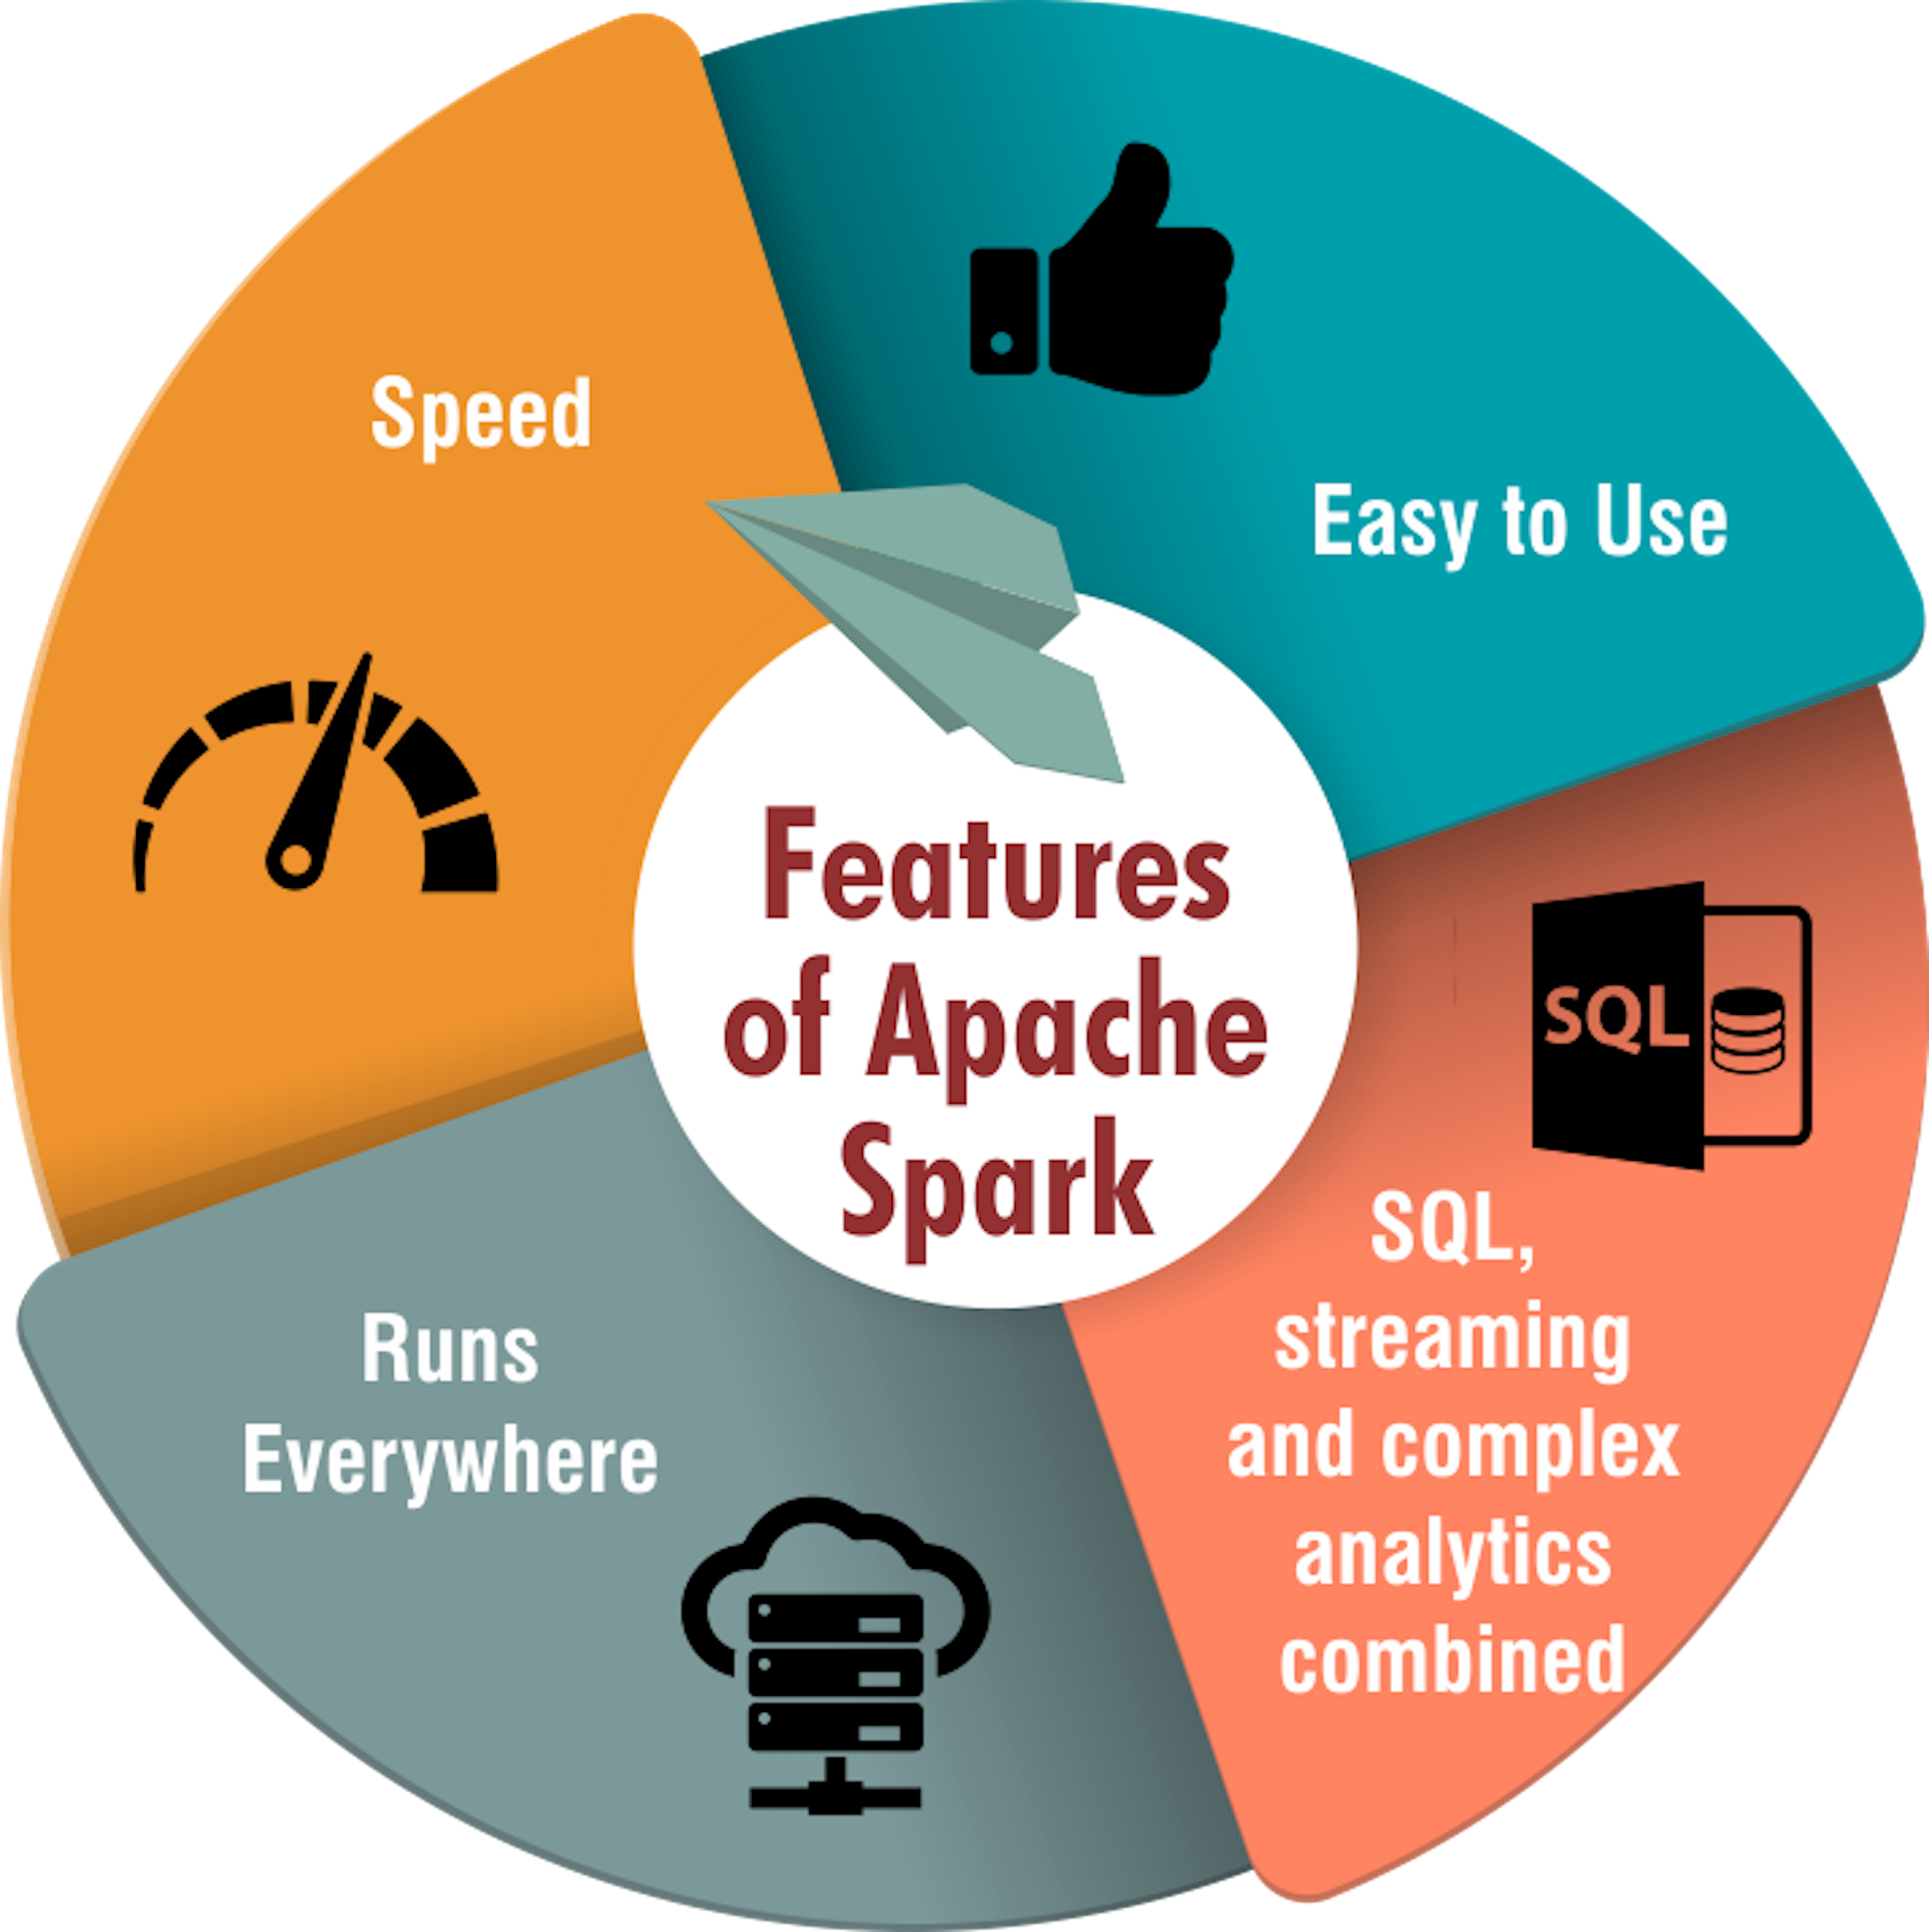
\includegraphics[height=3in]{/Users/viaandad/cloudmesh/hid-sp18-522/paper/Figures/sparkfeatures.png}
	\caption[Optional caption]{Real, Spak Features \cite{ref:feature}}
	\label{fig:sparkfeatures}
\end{figure}
\newpage
\section{Spark Engine}
Spark Core is the base engine for large-scale parallel and distributed data processing. It is responsible for: \hfill\break

\begin{itemize}
   \item  memory management and fault recovery
   \item  scheduling, distributing and monitoring jobs on a cluster
   \item  interacting with storage systems
\end{itemize}

Spark is built around  RDD (Resilient Distributed Dataset), an immutable fault-tolerant, distributed collection of objects that can be operated on in parallel. An RDD can contain any type of object and is created by loading an external dataset or distributing a collection from the driver program.
RDDs support two types of operations:\cite{ref:topal}\hfill\break

\begin{itemize}
   \item  Transformations are operations (such as map, filter, join, union, and so on) that are performed 		on an RDD and which yield a new RDD containing the result.
   \item  Actions are operations (such as reduce, count, first, and so on) that return a value after running a 		computation on an RDD.
\end{itemize}

Transformations in Spark are lazy, meaning that they do not compute their results right away. Instead, they just remember the operation to be performed and the dataset (e.g., file) to which the operation is to be performed. The transformations are only actually computed when an action is called, and the result is returned to the driver program. This design enables Spark to run more efficiently. For example, if a big file was transformed in various ways and passed to first action, Spark would only process and return the result for the first line, rather than do the work for the entire file.\cite{ref:topal} \hfill\break

By default, each transformed RDD may be recomputed each time you run an action on it. However, you may also persist an RDD in memory using the persist or cache method, in which case Spark will keep the elements around on the cluster for much faster access the next time you query it.\cite{ref:topal}\hfill\break

The Spark core comes bundled with some powerful libraries/components which could be seamlessly used in the same application. These libraries currently include SparkSQL, Spark Streaming, MLlib (for machine learning), and GraphX, each of which is further detailed in this article. Additional Spark libraries and extensions are currently under development as well.\cite{ref:topal}\hfill\break


\begin{figure}[H]
	\centering
	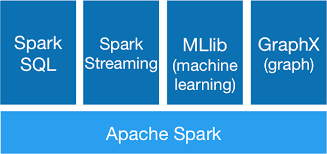
\includegraphics[height=2in]{/Users/viaandad/cloudmesh/hid-sp18-522/paper/Figures/Sparkarchitecture.png}
	\caption[Optional caption]{Spark Architecture}
	\label{fig:sparkfeatures}
\end{figure}

\subsection{SparkSQL}
SparkSQL is a Spark component that supports querying data either via SQL or via the Hive Query Language. It originated as the Apache Hive port to run on top of Spark (in place of MapReduce) and is now integrated with the Spark stack. In addition to providing support for various data sources, it makes it possible to weave SQL queries with code transformations which results in a very powerful tool. Below is an example of a Hive compatible query:\cite{ref:topal}\hfill\break

\begin{figure}[H]
	\centering
	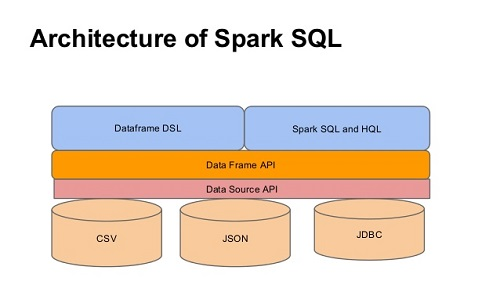
\includegraphics[height=3in]{/Users/viaandad/cloudmesh/hid-sp18-522/paper/Figures/sparksql.jpg}
	\caption[Optional caption]{Spark Sql Architecture\cite{ref:sql}}
	\label{fig:sparkfeatures}
\end{figure}

\subsection{Spark Streaming}
Spark Streaming supports real time processing of streaming data, such as production web server log files (e.g. Apache Flume and HDFS/S3), social media like Twitter, and various messaging queues like Kafka. Under the hood, Spark Streaming receives the input data streams and divides the data into batches.\cite{ref:topal} \hfill\break

\begin{figure}[H]
	\centering
	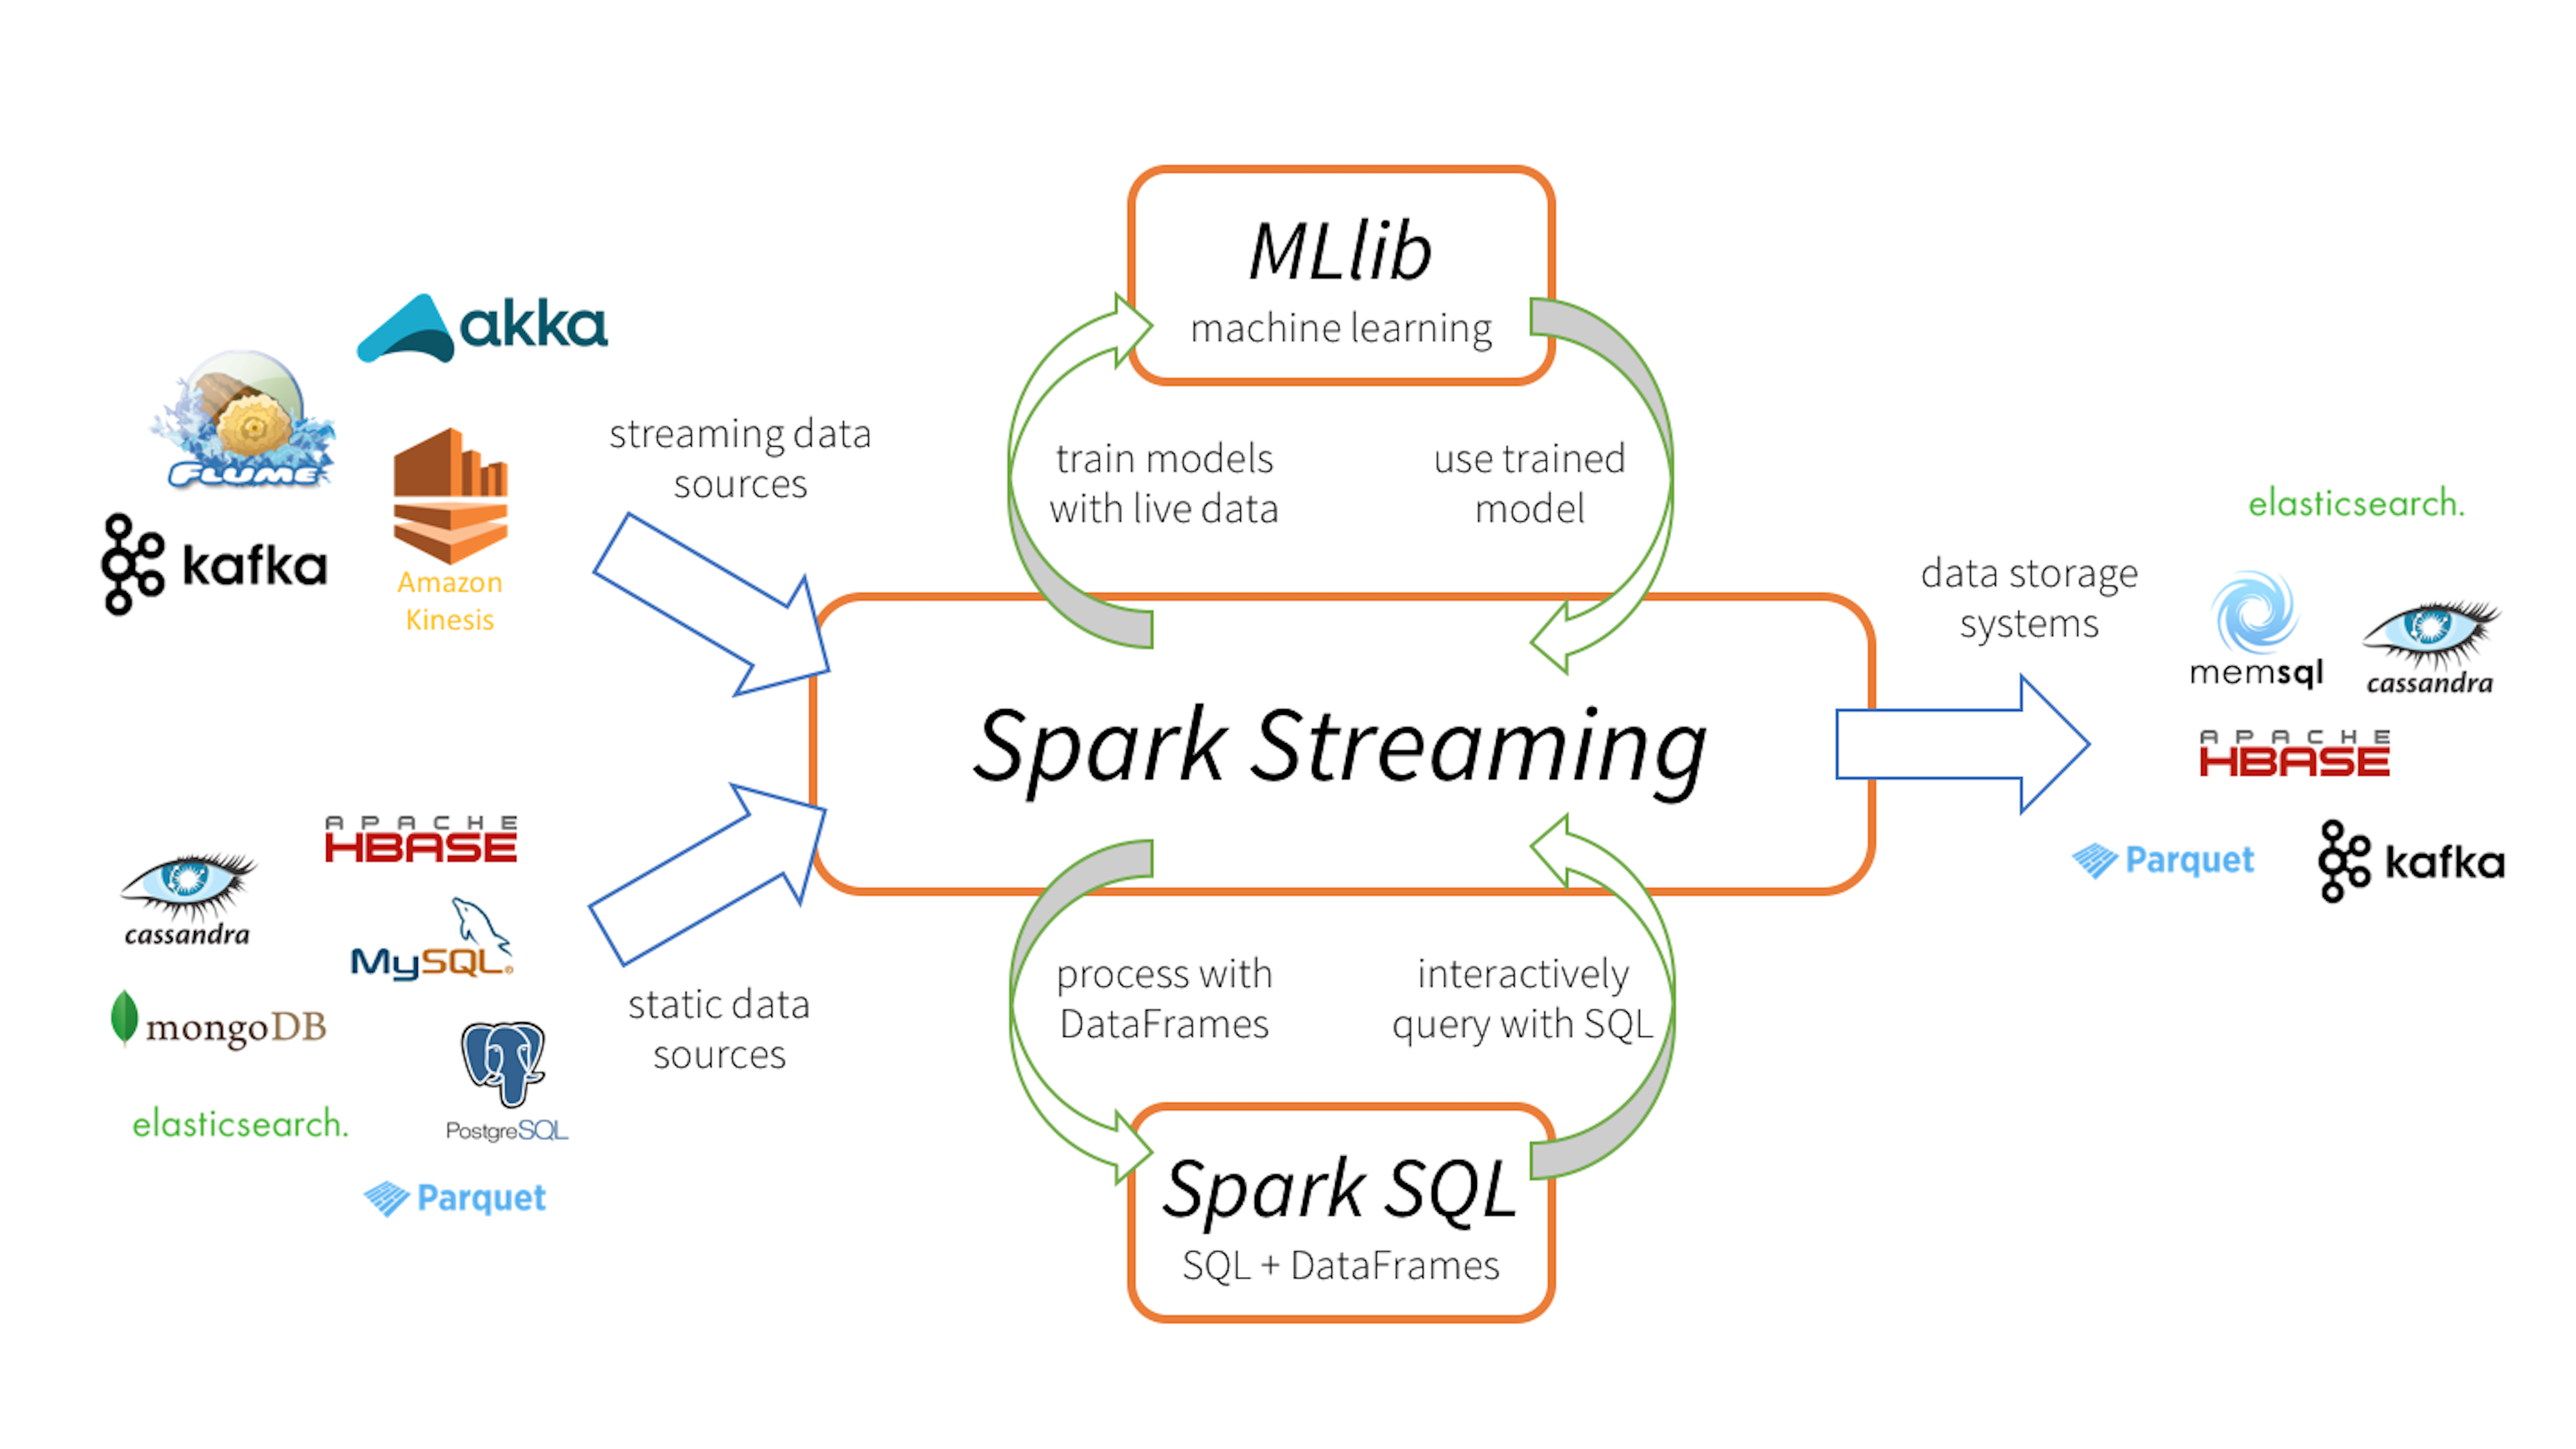
\includegraphics[height=3in]{/Users/viaandad/cloudmesh/hid-sp18-522/paper/Figures/sparkstream.png}
	\caption[Optional caption]{Spark Streaming  \cite{ref:databricks}}
	\label{fig:sparkfeatures}
\end{figure}

\subsection{MLlib}
MLlib is Spark's open-source distributed machine learning library. MLlib provides efficient functionality for a wide range of learning settings and includes several underlying statistical, optimization, and linear algebra primitives. Shipped with Spark, MLlib supports several languages and provides a high-level API that leverages Spark's rich ecosystem to simplify the development of end-to-end machine learning pipelines. MLlib has experienced a rapid growth due to its vibrant open-source community of over 140 contributors, and includes extensive documentation to support further growth and to let users quickly get up to speed\cite{ref:spark}\hfill\break

\begin{figure}[H]
	\centering
	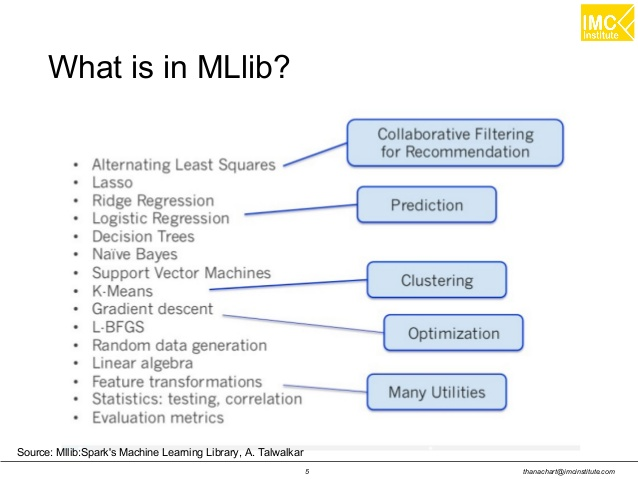
\includegraphics[height=3in]{/Users/viaandad/cloudmesh/hid-sp18-522/paper/Figures/mlib.jpg}
	\caption[Optional caption]{Mlib \cite{ref:databricks}}
	\label{fig:sparkfeatures}
\end{figure}

\subsection{GraphX}
GraphX is a new component in Spark for graphs and graph-parallel computation. At a high level, GraphX extends the Spark RDD by introducing a new Graph abstraction: a directed multigraph with properties attached to each vertex and edge. To support graph computation, GraphX exposes a set of fundamental operators (e.g., subgraph, join Vertices, and aggregate Messages) as well as an optimized variant of the Pregel API. In addition, GraphX includes a growing collection of graph algorithms and builders to simplify graph analytics tasks.\cite{ref:graphx}\hfill\break

\section{Other Apache Spark Use Cases}

\subsection{Gaming Industry}
In the game industry, processing and discovering patterns from the potential firehose of real-time in-game events and being able to respond to them immediately is a capability that could yield a lucrative business, for purposes such as player retention, targeted advertising, auto-adjustment of complexity level, and so on.\cite{ref:deepcore}\hfill\break

\subsection{Finance Industry}

In the finance or security industry, the Spark stack could be applied to a fraud or intrusion detection system or risk-based authentication. It could achieve top-notch results by harvesting huge amounts of archived logs, combining it with external data sources like information about data breaches and compromised accounts and information from the connection/request such as IP geolocation or time.\cite{ref:deepcore}\hfill\break

\subsection{IoT}
IoT is rapidly emerging as a leading area for Apache Spark applications. In the real-world data analysis pipelines, where real-time streams are collected from edge devices, gateways, or other clouds, and then processed by Spark Streaming applications, which in turn generate derived streams for further processing, data aggregates, or trigger other real-time events. Spark's capability of using similar code for both stream and batch processing can simplify a number of data management issues. Modern IoT operations can drive digital transformation by analyzing the unprecedented amounts of data generated from devices and sensors in real-time.\cite{ref:IoT}\hfill\break

Apache Spark is a widely used stream processing engine for real-time IoT applications. Spark streaming offers a rich set of APIs in the areas of ingestion, cloud integration, multi-source joins, blending streams with static data, time-window aggregations, transformations, data cleansing, and strong support for machine learning and predictive analytics.\cite{ref:deepcore}\hfill\break

\cleardoublepage
\bibliographystyle{IEEEtran}
\bibliography{/Users/viaandad/cloudmesh/hid-sp18-522/paper/Reference/references}





\end{document}

